\documentclass[10pt,twocolumn,letterpaper]{article}

\usepackage{cvpr}
\usepackage{times}
\usepackage{epsfig}
\usepackage{graphicx}
\usepackage{amsmath}
\usepackage{amssymb}

\def\cvprPaperID{1} % *** Enter the CVPR Paper ID here

\usepackage[breaklinks=true,bookmarks=false]{hyperref}

\cvprfinalcopy % Comment this line and it stop working! :(
\ifcvprfinal\pagestyle{empty}\fi

\def\httilde{\mbox{\tt\raisebox{-.5ex}{\symbol{126}}}}

% Pages are numbered in submission mode, and unnumbered in camera-ready
%\ifcvprfinal\pagestyle{empty}\fi
\setcounter{page}{1}

\graphicspath{ {./images/} } 

\sloppy

%-------------------------------------------------------------------------
%-------------------------------------------------------------------------

\begin{document}

%%%%%%%%% TITLE
\title{\textit{Project Milestone:} Convolutional Neural Network to Image Segmentation}

\author{Felipe Augusto Lima Reis\\
PUC Minas - Pontif\'icia Universidade Cat\'olica de Minas Gerais\\
R. Walter Ianni 255 - Bloco L - Belo Horizonte, MG, Brasil\\
{\tt\small falreis@sga.pucminas.br}
}

\maketitle
%\thispagestyle{empty}

%%%%%%%%% ABSTRACT
\begin{abstract}
    Image segmentation refers to the partition of an image into a set of regions to cover it, to represent a meaningful area. The future paper will evaluate segmentation methods using Deep Neural Networks and compares with classical methods of segmentation, using the superpixels approach. Also, the paper will evaluate the composition of classical methods with DNN approach, to speed up the training process and become more accurate.
\end{abstract}

%%%%%%%%% BODY TEXT
\section{Introduction} \label{introduction}

Image segmentation refers to the partition of an image into a set of regions to cover it, to represent meaningful areas \cite{DOMINGUEZ}. The goal is to simplify and/or change the representation of an image into something
that is more meaningful and easier to analyze \cite{AHMED_SARMA}.

Segmentation has two main objectives: the first one is to decompose the image into parts for further analysis and the second one is to perform a change of representation \cite{DOMINGUEZ}. Also, segmentation must follow some characteristics to identify regions, as it follows:

\begin{itemize}
 \item Regions of an image segmentation should be uniform and homogeneous with respect to some characteristic, such as gray level, color, or texture \cite{DOMINGUEZ};
 \item Region interiors should be simple and without many small holes \cite{DOMINGUEZ};
 \item Adjacent regions of a segmentation should have significantly different values with respect to the characteristic on which they are uniform \cite{DOMINGUEZ};
 \item Boundaries of each segment should be smooth, not ragged, and should be spatially accurate \cite{DOMINGUEZ}.
\end{itemize}

The future paper will evaluate segmentation methods using Deep Neural Networks and compares with classical methods of segmentation, using the superpixels approach. Also, the paper will evaluate the composition of classical methods with DNN approach, to speed up the training process and become more accurate.

The organization of this paper is as follows. In the next Section we discuss the problem statement. Section \ref{sec:tech_approach} explains how the will work and the results we expect.

%-------------------------------------------------------------------------
\section{Problem Statement} \label{sec:prob_statement}

%Describe your problem precisely specifying the dataset to be used, expected results and evaluation

Semantic pixel-wise segmentation is an active topic of research \cite{SEGNET}. Before the use of deep neural networks, the  best-performing methods mostly was made using hand engineered features \cite{SEGNET}.

The success of deep convolutional neural networks for object classification led researchers to use these techniques to learn new capabilities, such as segmentation \cite{SEGNET}. 

The future paper will evaluate some Deep Neural Networks to segmentation, as SEGNET \cite{SEGNET} and U-NET \cite{UNET}, and compare to classical methods, like SLIC (Simple Linear Iterative Clustering) \cite{SLIC} and EGB (Efficient Graph-Based Image Segmentation) \cite{FELZENSZWALB}. For this, it will be used Berkeley Segmentation Data Set 500 (BSDS500) \cite{BSDS500}.

Berkeley Segmentation Data Set contains 500 natural images and its respective ground-truths, annotated by humans \cite{BSDS500}. The images are explicitly separated into disjoint train, validation and test subsets \cite{BSDS500}.

To evaluate the quality of the segmentation methods, the results will be evaluated with BSDS500 benchmarking tool, provided with the Dataset \cite{BSDS500}. BSDS500 dataset uses the Precision and Recall Method to evaluate the results \cite{BSDS500}.

This work expects better performance of Deep Neural Network when compared with classical methods (SLIC and EGB). The results must be more precise, but with time and space complexity bigger then classical algorithms. 

%-------------------------------------------------------------------------
\section{Technical Approach} \label{sec:tech_approach}

%Describe the methods you intend to apply to solve the given problem

This section contains the technical approach to reach the goals explained in Section \ref{sec:prob_statement}.

%-------------------------------------------------------------------------
\subsection{Deep Neural Networks} \label{ssec:neura_nets}

The project will use two different Neural Networks to provide segmentation, as it follows in the next subsections.

%-------------------------------------------------------------------------
\subsubsection{SEGNET} \label{sssec:segnet}

SEGNET is a deep encoder-decoder architecture for multi-class pixelwise segmentation \cite{SEGNET}. The SEGNET architecture consists of a sequence of non-linear processing layers (encoders) and a corresponding set of decoders followed by a pixel-wise classifier \cite{SEGNET} \cite{SEGNET_WEBSITE}. Typically, each encoder consists of one or more convolutional layers with batch normalization and a ReLU non-linearity, followed by non-overlapping max-pooling and sub-sampling \cite{SEGNET} \cite{SEGNET_WEBSITE}. The sparse encoding due to the pooling process is upsampled in the decoder using the max-pooling indices in the encoding sequence \cite{SEGNET} \cite{SEGNET_WEBSITE}. Figure \ref{fig:segnet} presents the architecture of SEGNET.

\begin{figure}[ht]
  \centering
  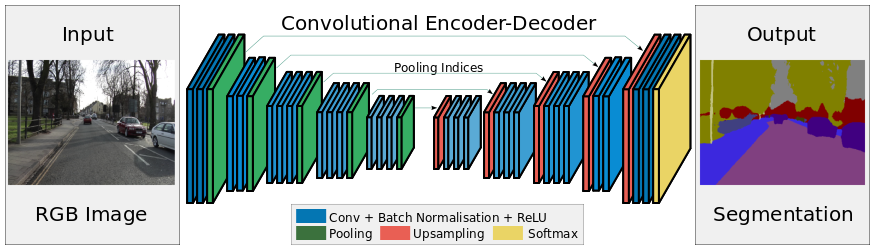
\includegraphics[width=0.48\textwidth]{segnet.png}
  \caption{SEGNET architecture. \textit{Image adapted from SEGNET project website} \cite{SEGNET_WEBSITE} \cite{SEGNET}}
  \label{fig:segnet}
\end{figure}


%-------------------------------------------------------------------------
\subsubsection{U-NET} \label{sssec:unet}

U-NET is a Convolutional Networks for Biomedical Image Segmentation \cite{UNET} \cite{UNET_WEBSITE}. Although U-NET was developed for biomedical image segmentation, its architecture can be trained to segment other types of image. In this project, we will use U-NET to classify images from BSDS500.

U-NET architecture consists of the repeated application of two $3 \times 3$ convolutions, each followed by a rectified linear unit (ReLU) and a $2 \times 2$ max pooling operation with stride 2 for downsampling \cite{UNET}. Every step in the expansive path consists of an upsampling of the feature map followed by a $2 \times 2$ convolution, a concatenation with the correspondingly cropped feature map from the contracting path, and two $3 \times 3$ convolutions, each followed by a ReLU \cite{UNET}. At the final layer a $1 \times 1$ convolution is used. In total the network has 23 convolutional layers \cite{UNET}. Figure \ref{fig:unet} presents the  architecture of U-NET.

\begin{figure}[ht]
  \centering
  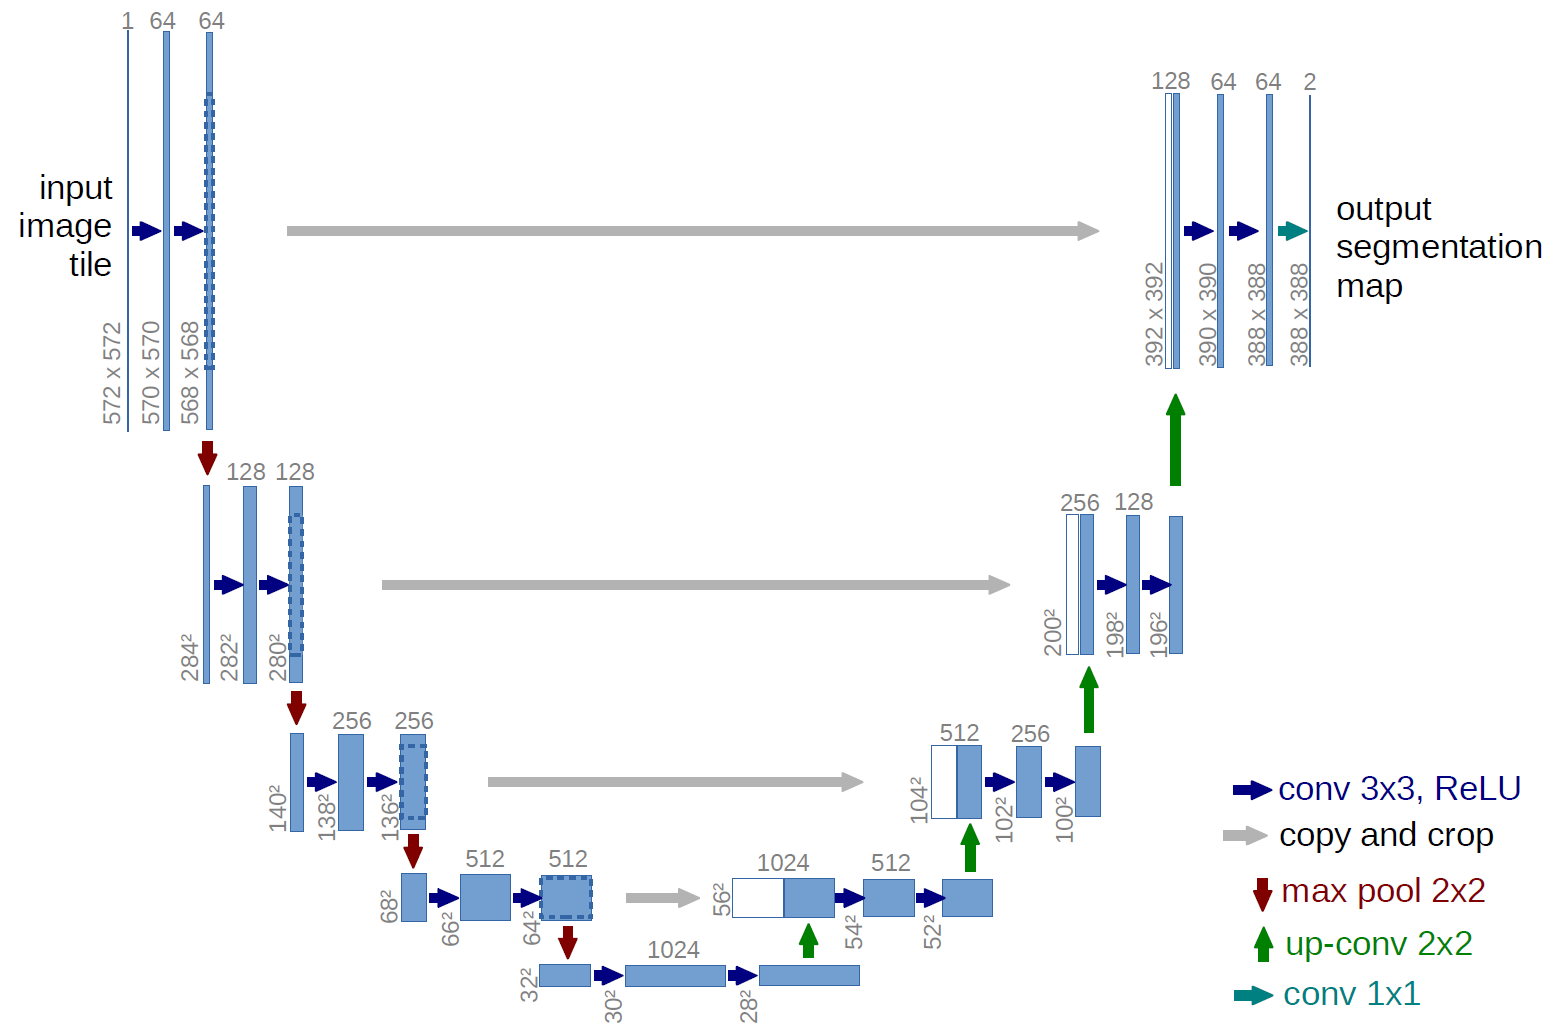
\includegraphics[width=0.48\textwidth]{unet.png}
  \caption{U-NET architecture. \textit{Image adapted from U-NET project website} \cite{UNET_WEBSITE} \cite{UNET}}
  \label{fig:unet}
\end{figure}

%-------------------------------------------------------------------------
\subsection{Transfer Learning} \label{ssec:transfer_learning}

Transfer learning is a technique in machine learning that stores knowledge gained while solving one problem, adapt and apply it to a different but related problem. As the growing of neural networks usage, it becomes reasonable to seek out methods that avoid ``reinventing the wheel'', and instead are able to build on previously trained networks' results \cite{PRATT} \cite{WEISS2016}.

In this work is expected to use transfer learning to speed up the training process. For that, it will be used a pre-trained VGG-16 (Very Deep Convolutional Networks for Large-Scale Image Recognition) \cite{VGGNET}. The pre-trained VGG-16 will be provided by Keras, a Python Deep Learning Library \cite{KERAS}. Keras is a high-level neural networks API of running on top of TensorFlow \cite{TENSORFLOW}, CNTK \cite{CNTK}, or Theano \cite{THEANO} \cite{KERAS}.

VGG-16 provided by Keras contains weights pre-trained on ImageNet Dataset \cite{IMAGENET}. ImageNet contains a fixed-size 224 × 224 RGB image. VGG-16 passes the image through a stack of convolutional (conv.) layers, where it's used filters with a very small receptive field: $3 \times 3$ \cite{VGGNET}. The convolution stride is fixed to 1 pixel and the spatial padding of convolutional layer input is such that the spatial resolution is preserved after convolution \cite{VGGNET}. Spatial pooling is carried out by five max-pooling layers, which follow some of the convolutional layers \cite{VGGNET}. Max-pooling, them, is performed over a $2 \times 2$ pixel window, with stride 2 \cite{VGGNET}. Figure \ref{fig:vgg16} presents the architecture of VGG-16.

\begin{figure}[ht]
  \centering
  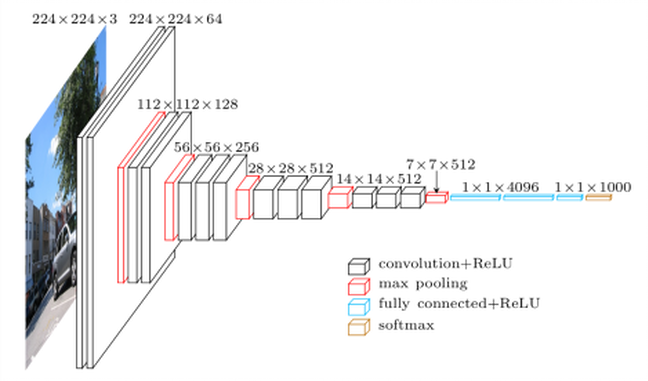
\includegraphics[width=0.48\textwidth]{vgg16.png}
  \caption{VGG-16 architecture. \textit{Image adapted from TechKingdom website\cite{VGG16_IMG}}}
  \label{fig:vgg16}
\end{figure}

To use transfer learning, it will be needed to make some data transformations. First, it will need to adapt SEGNET architecture to uses VGG-16 weights. Also, the BSDS500 images and ground-truths will be reduced to the shape of $ 224 \times 224$. As BSDS500 images are not square, a process step will transform the shape, adding black borders before reducing the image. This step will avoid deformations in the shape of the image and the ground-truth.

%-------------------------------------------------------------------------
\subsection{Data Augmentation} \label{ssec:data_augmentation}

Data augmentation consists of a range of transformations that can be applied to the dataset to increase the number of data with the target of improving the accuracy and robustness of classifiers \cite{AUGM_ADAPT}. The problem with small datasets is that models trained with them do not generalize well \cite{AUGM_DEEP}.

Data augmentation also can act as a regularizer in preventing overfitting in neural networks and improve performance in imbalanced class problems \cite{DATA_AUGM}. According to Wong et al. \cite{DATA_AUGM}, data augmentation is better to perform in data-space instead of feature-space, as long as label preserving transforms are known \cite{DATA_AUGM}.

Once BSDS500 contains only 200 images for training and 100 images for validation, the Neural Network may not generalize well and learn enough information from the dataset. Then, it's necessary to provide a range of transformation to add some generated images for training and validation.

To provide data augmentation, the images and the ground-truth will be rotated 12 times, 30 degrees each. Also, the images will be flipped and rotated 12 times each. Then, each image will transform into 24 possible images. Then, 200 images for the training set will become 4800 training images and the validation set will contains 2400 images. The number of images is not too big but can help the DNN predict with more accuracy.

%-------------------------------------------------------------------------

{\small
\bibliographystyle{ieee}
\bibliography{egbib}
}

\end{document}
